% !TeX program = xelatex
% =====================================================================
%  FPP paper v4 -- BAN TU CHUA (standalone), khong can IEEEtran.cls
%  Dinh dang theo yeu cau mon hoc:
%    Times New Roman 10pt | can deu | 2 cot | column spacing 0.25 in
%    Danh so muc kieu IEEE: I, II, ... va A, B, ...
%  Compile: XeLaTeX (BAT BUOC - de hien thi dau tieng Viet trong ten tac gia)
%           Chay 2-3 lan de cap nhat tham chieu bang/hinh
%  Can 4 file hinh: rfig1_accuracy.png ... rfig4_perobj.png
% =====================================================================
\documentclass[10pt,twocolumn,letterpaper]{article}

% ---------- trang & cot ----------
\usepackage[letterpaper,top=0.75in,bottom=1.0in,left=0.625in,right=0.625in]{geometry}
\setlength{\columnsep}{0.25in}          % yeu cau: ~0.25 inch

% ---------- font Times ----------
% Font Times ho tro day du dau tieng Viet (bien dich bang XeLaTeX hoac LuaLaTeX)
\usepackage{fontspec}
\setmainfont{TeX Gyre Termes}          % ban Times chuan, co day du dau tieng Viet
\usepackage{unicode-math}
\setmathfont{TeX Gyre Termes Math}

% ---------- goi ----------
\usepackage{amsmath}
\usepackage{graphicx}
\graphicspath{{figures/}}   % hinh nam trong thu muc figures/
\usepackage{booktabs}
\usepackage{array}
\usepackage{cite}
\usepackage[font=small,labelfont=bf,justification=raggedright,singlelinecheck=false]{caption}
\usepackage{titlesec}
\usepackage{indentfirst}

% ---------- kieu danh so muc IEEE ----------
\renewcommand{\thesection}{\Roman{section}}
\renewcommand{\thesubsection}{\Alph{subsection}}
\titleformat{\section}[block]{\centering\normalsize\scshape}{\thesection.}{0.5em}{}
\titleformat{\subsection}[block]{\normalsize\itshape}{\thesubsection.}{0.5em}{}
\titlespacing*{\section}{0pt}{10pt}{4pt}
\titlespacing*{\subsection}{0pt}{6pt}{2pt}

% ---------- caption kieu IEEE ----------
\renewcommand{\figurename}{Fig.}
\captionsetup[table]{name=TABLE,labelsep=newline,justification=centering,textfont=sc}
\renewcommand{\thetable}{\Roman{table}}

% ---------- doan van ----------
\setlength{\parindent}{1em}
\setlength{\parskip}{0pt}
\raggedbottom

% ---------- tuong thich lenh IEEEtran ----------
\newcommand{\IEEEauthorblockN}[1]{{\normalsize #1}\par\vspace{2pt}}
\newcommand{\IEEEauthorblockA}[1]{{\small\itshape #1}\par}
\newenvironment{IEEEkeywords}{\vspace{4pt}\noindent\small\textbf{\textit{Index Terms}}---}{\par\vspace{4pt}}

% ---- dieu chinh vi tri float: cho phep nhieu float/trang, uu tien gan van ban ----
\setcounter{topnumber}{3}
\setcounter{bottomnumber}{2}
\setcounter{totalnumber}{4}
\renewcommand{\topfraction}{0.92}
\renewcommand{\bottomfraction}{0.75}
\renewcommand{\textfraction}{0.06}
\renewcommand{\floatpagefraction}{0.70}
\setlength{\floatsep}{7pt plus 2pt minus 2pt}
\setlength{\textfloatsep}{9pt plus 2pt minus 2pt}
\setlength{\intextsep}{7pt plus 2pt minus 2pt}

\begin{document}
\newcommand{\PAPERTITLE}{Farthest-Point Hypothesis Pruning for Fast\\ Frame-0 Registration in FoundationPose}
\newcommand{\PAPERAUTHOR}{\IEEEauthorblockN{Hoàng Minh Khoa, Phạm Đức Dương, Nguyễn Đình Cao Minh,\\ Trần Hữu Lộc, Nguyễn Gia Bình}
\IEEEauthorblockA{Department of Electrical and Computer Engineering\\
Vietnamese-German University (VGU)\\
Technical Writing --- Group 40}}
\twocolumn[
\begin{@twocolumnfalse}
\vspace*{-6pt}
\begin{center}
{\LARGE\bfseries Farthest-Point Hypothesis Pruning for Fast\\ Frame-0 Registration in FoundationPose\par}\vspace{8pt}
{\normalsize Hoàng Minh Khoa, Phạm Đức Dương, Nguyễn Đình Cao Minh, Trần Hữu Lộc, Nguyễn Gia Bình\par}\vspace{3pt}
{\small\itshape Department of Electrical and Computer Engineering\\
Vietnamese-German University (VGU)\\
Technical Writing --- Group 40\par}
\end{center}
\vspace{10pt}
\end{@twocolumnfalse}
]

% ---- Abstract nam o file rieng ----
% =====================================================================
%  ABSTRACT -- file rieng, duoc main.tex goi bang  % =====================================================================
%  ABSTRACT -- file rieng, duoc main.tex goi bang  % =====================================================================
%  ABSTRACT -- file rieng, duoc main.tex goi bang  \input{abstract}
%  Sua noi dung abstract ngay tai day.
% =====================================================================
\noindent\small\textbf{\textit{Abstract}} --- FoundationPose registers a novel object on the first video frame by refining and scoring a fixed grid of 252 pose hypotheses; this step dominates initialization latency. This study focuses on how few hypotheses are needed and how they should be selected. From a fixed pool of 504 rendered templates, this paper compares three selection strategies which are uniform random, geodesic farthest-point sampling (FPS), and DINOv2 bag-of-words retrieval. These strategies feed the same FoundationPose refiner and scorer, and are evaluated on 21 YCB-Video objects with ADD/ADD-S against ground truth. Against the full 252-hypothesis grid, FPS with $K{=}20$ reaches 97.5\% ADD-S against the grid's 98.8\% at about nine times lower latency, and matches it exactly (98.8\%) at $K{=}50$; across all 21 objects it attains 99.4\% at $K{=}20$. In contrast, DINOv2 bag-of-words retrieval underperforms even random selection for $K \ge 5$, because bag-of-words ranking is not viewpoint-discriminative and concentrates hypotheses by appearance rather than covering the rotation space. Registration time follows $t \approx 192 + 17.0K$ ms. We provide operating recommendations and a failure analysis on small and symmetric objects.
\par\vspace{4pt}

%  Sua noi dung abstract ngay tai day.
% =====================================================================
\noindent\small\textbf{\textit{Abstract}} --- FoundationPose registers a novel object on the first video frame by refining and scoring a fixed grid of 252 pose hypotheses; this step dominates initialization latency. This study focuses on how few hypotheses are needed and how they should be selected. From a fixed pool of 504 rendered templates, this paper compares three selection strategies which are uniform random, geodesic farthest-point sampling (FPS), and DINOv2 bag-of-words retrieval. These strategies feed the same FoundationPose refiner and scorer, and are evaluated on 21 YCB-Video objects with ADD/ADD-S against ground truth. Against the full 252-hypothesis grid, FPS with $K{=}20$ reaches 97.5\% ADD-S against the grid's 98.8\% at about nine times lower latency, and matches it exactly (98.8\%) at $K{=}50$; across all 21 objects it attains 99.4\% at $K{=}20$. In contrast, DINOv2 bag-of-words retrieval underperforms even random selection for $K \ge 5$, because bag-of-words ranking is not viewpoint-discriminative and concentrates hypotheses by appearance rather than covering the rotation space. Registration time follows $t \approx 192 + 17.0K$ ms. We provide operating recommendations and a failure analysis on small and symmetric objects.
\par\vspace{4pt}

%  Sua noi dung abstract ngay tai day.
% =====================================================================
\noindent\small\textbf{\textit{Abstract}} --- FoundationPose registers a novel object on the first video frame by refining and scoring a fixed grid of 252 pose hypotheses; this step dominates initialization latency. This study focuses on how few hypotheses are needed and how they should be selected. From a fixed pool of 504 rendered templates, this paper compares three selection strategies which are uniform random, geodesic farthest-point sampling (FPS), and DINOv2 bag-of-words retrieval. These strategies feed the same FoundationPose refiner and scorer, and are evaluated on 21 YCB-Video objects with ADD/ADD-S against ground truth. Against the full 252-hypothesis grid, FPS with $K{=}20$ reaches 97.5\% ADD-S against the grid's 98.8\% at about nine times lower latency, and matches it exactly (98.8\%) at $K{=}50$; across all 21 objects it attains 99.4\% at $K{=}20$. In contrast, DINOv2 bag-of-words retrieval underperforms even random selection for $K \ge 5$, because bag-of-words ranking is not viewpoint-discriminative and concentrates hypotheses by appearance rather than covering the rotation space. Registration time follows $t \approx 192 + 17.0K$ ms. We provide operating recommendations and a failure analysis on small and symmetric objects.
\par\vspace{4pt}


\noindent\small\textbf{\textit{Index Terms}} --- 6D object pose estimation, FoundationPose, hypothesis pruning, farthest-point sampling, DINOv2, render-and-compare, YCB-Video.
\par\normalsize\vspace{6pt}

\section{Introduction}

\subsection{Background and Motivation}
Six-degree-of-freedom (6D) object pose estimation determines the rotation and translation that align an object's frame with the camera frame, and underpins robotic manipulation as well as augmented reality. FoundationPose [1] estimates the pose of a novel object without retraining and reached first place on the model-based ``Benchmark for 6D Object Pose estimation'' (BOP) leaderboard upon release. The system performs pose estimation only on the first frame of video, which is termed registration. Thus, registration latency determines the response speed of the pipeline as well as the cost of dataset-scale evaluation. Registration is expensive because a fixed grid of 252 pose hypotheses is passed through a refinement network and a scoring network, and both are evaluated for every hypothesis. The grid is identical for every scene, so most of its hypotheses are far from the true pose but are refined and scored anyway.

\subsection{Literature Survey}
Render-and-compare methods estimate the pose of novel objects by comparing renderings of its model with the observation; MegaPose [2] and FoundationPose [1] are representative, and FoundationPose reconstructs a model-free object from reference views using a neural field derived from BundleSDF [3]. A second family selects a coarse pose from templates using features of 2D foundation models: FoundPose [4] ranks rendered templates with DINOv2 [5] descriptors through a bag-of-words index in the tradition of Video Google [6], and GigaPose [7] matches templates by patch correspondence. Accuracy is measured by ``Average Distance'' (ADD) [8], introduced for texture-less objects, and its symmetry-aware variant ``Average Distance for Symmetry'' (ADD-S) [9], adopted in the BOP protocol [10], on datasets such as YCB-Video [9].

\subsection{Research Gap}
FoundationPose draws its first-frame hypotheses from an object-independent grid of 252 rotations, refines then scores all of them. This leaves two open questions: how many hypotheses are required, and how they should be chosen. FoundationPose has a very strong refiner, but the hypotheses fed into it do not depend on the image at all: every scene uses the same 252 rotations, and all 252 are refined and scored. Foundation-feature retrieval methods are the other way round. They do use the observation to propose poses, but they are only run as the final estimator, with no refiner behind them. No work has used them as a selection stage to decide which hypotheses go into the refiner and scorer. This paper puts the two together: a selector that chooses a small set of hypotheses, and FoundationPose's refiner and scorer to turn them into a pose.

\subsection{Contributions}
(1) This paper shows that first-frame registration cost scales linearly with the number of hypotheses and validate the time model $t \approx c_0 + c_1K$.

(2) Comparing three hypothesis-selection strategies: random, geodesic FPS, and DINOv2 bag-of-words retrieval over 504 templates of 21 YCB-Video objects with an identical refiner and scorer.

(3) FPS achieves 97.5\% ADD-S versus the full grid's 98.8\% on a matched object set at about ninefold lower latency, and reaches it exactly at $K{=}50$.

(4) DINOv2 bag-of-words retrieval underperforms even random selection, and we explain it by the viewpoint-blind nature of bag-of-words.

(5) We give operating recommendations and a failure analysis.

\section{System Model}

\subsection{Characteristics and Assumptions}
The input is a single RGB-D frame from a calibrated camera, with a mask and a textured mesh of the rigid target object.

Each assumption has a practical basis. RGB-D input with calibrated intrinsics is the standard sensing configuration on manipulation platforms, and depth enables a metric translation estimate from a single view. Rigidity holds for the graspable household objects targeted here, so a single 6D transform fully describes the object state. A textured mesh is available in the model-based setting either from a CAD library or, in the model-free setting, from a few reference views. The first-frame mask is required for FoundationPose, which we use as the baseline to compare hypothesis-selection strategies; retaining it keeps the comparison faithful and confines the study to the hypothesis-selection stage, ensuring the comparison is not confounded by multiple changes to the input data at the same time.

The methods studied here differ only in which pose hypotheses are fed into the refiner. The object model, mask, networks, and evaluation metrics are all held fixed. Notation is listed in Table~\ref{tab:notation}.

\begin{table}[tb]
\caption{Notation}
\label{tab:notation}
\centering\small
\begin{tabular}{@{}ll@{}}
\toprule
Symbol & Description \\
\midrule
$T=[R\,|\,t]$ & object-to-camera pose, $R\in SO(3)$ \\
$N$ & full-grid hypotheses ($N = 252$) \\
$P$ & template pool ($|P| = 504$) \\
$K$ & retained hypotheses \\
$c_0$ & fixed pre-processing cost \\
$c_1$ & per-hypothesis refine+score cost \\
$d(R_a, R_b)$ & geodesic rotation distance \\
$\mathcal{M}$ & object model point set \\
$d_{\mathrm{diam}}$ & object diameter \\
\bottomrule
\end{tabular}
\end{table}

\subsection{Mathematical Model}
Registration returns $T = [R\,|\,t]$, $R \in SO(3)$, $t \in \mathbb{R}^3$. FoundationPose builds a hypothesis set of $N = 252$ rotations, refines each with a network over five iterations, scores them, and returns the best. Since both networks run on every hypothesis, the time is
\begin{equation}
t_{\mathrm{reg}} \approx c_0 + c_1 N,
\end{equation}
where $c_1$ is the per hypothesis refine and score cost. Pruning to $K \ll N$ hypotheses gives $t_{\mathrm{reg}} \approx c_0 + c_1 K$. We draw the $K$ hypotheses from a fixed pool $P$ of 504 pre-rendered template poses; the pool is identical for all strategies, so only the selection differs. Geodesic distance between two rotations is
\begin{equation}
d(R_a,R_b)=\arccos\!\Big(\tfrac{\operatorname{tr}(R_a^{\top}R_b)-1}{2}\Big).
\end{equation}
Accuracy uses the average distance over the model points $\mathcal{M}$,
\begin{equation}
e_{\mathrm{ADD}}=\frac{1}{|\mathcal{M}|}\sum_{x\in\mathcal{M}}\big\lVert(Rx+t)-(R^\star x+t^\star)\big\rVert,
\end{equation}
and the symmetric variant $e_{\mathrm{ADD\text{-}S}}$ replaces the term by the distance to the nearest model point of the transformed model; a pose is considered correct when $e < 0.1\,d_{\mathrm{diam}}$. ADD-S is the primary metric because many YCB objects are symmetric.

\subsection{Dataset}
We use YCB-Video [9], specifically adopting the ref\_views\_16 subset standard in FoundationPose: 21 object meshes with ground-truth 6D poses. Each object is evaluated on 16 frames. The annotated convention is auto-detected once per run by matching the full-grid output rotation against the annotation and its inverse. ADD-S diameters are computed from the convex hull; ADD uses 3000 sampled model points. The 21 objects are shown in Fig.~\ref{fig:objects}.

\begin{figure}[tb]
\centering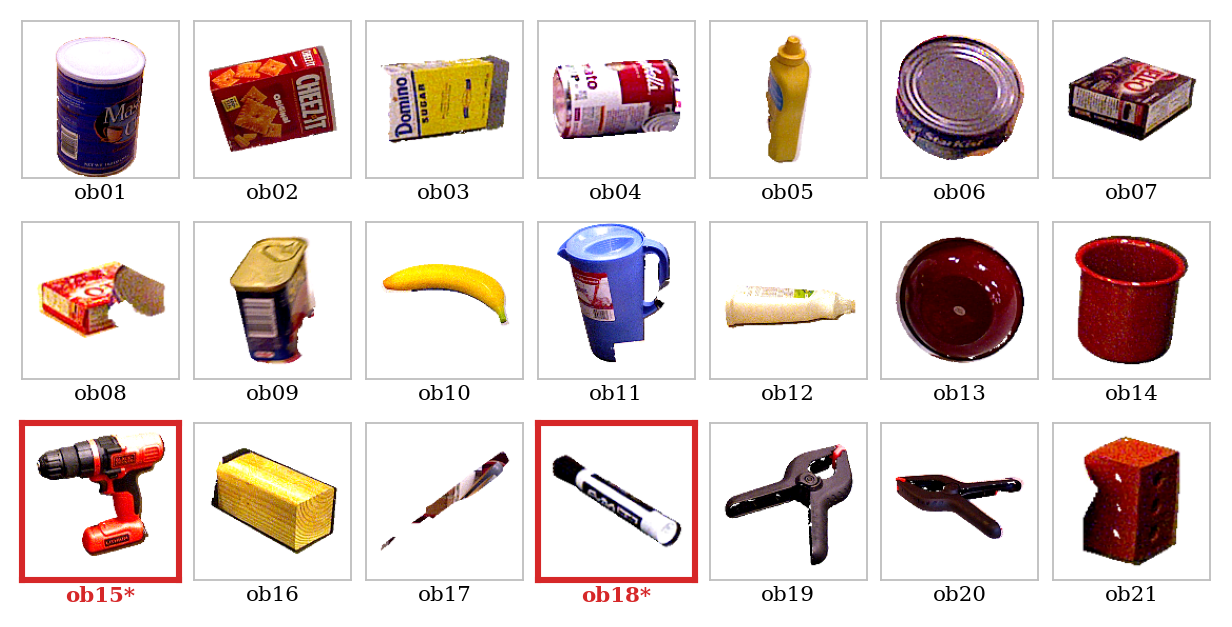
\includegraphics[width=\columnwidth]{rfig5_objects.png}
\caption{The 21 YCB-Video objects used in the evaluation (reference views, background removed). The two objects marked in red (ob15, a power drill; ob18, a marker pen) are the only ones that stay below 100\% ADD-S at farthest $K{=}20$.}
\label{fig:objects}
\end{figure}

\begin{table}[tb]
\centering\small
\renewcommand{\arraystretch}{1.15}
\begin{tabular}{@{}p{0.95\columnwidth}@{}}
\toprule
\textbf{Algorithm 1}~~Geodesic Farthest-Point Hypothesis Selection \\
\midrule
\textbf{Input:} pool rotations $\{R_i\}_{i=1}^{504}$, budget $K$ \\
1: $S \leftarrow \{\,\text{random index}\,\}$ \\
2: $m_i \leftarrow d(R_i,R_{S_1})$ for all $i$ \\
3: \textbf{for} $j=2$ \textbf{to} $K$: \\
4: \quad $n \leftarrow \arg\max_i m_i$;\; $S \leftarrow S\cup\{n\}$ \\
5: \quad $m_i \leftarrow \min(m_i,\,d(R_i,R_n))$ for all $i$ \\
6: \textbf{return} pool poses indexed by $S$ \\
\bottomrule
\end{tabular}
\end{table}

\subsection{Models for Fair Comparison}
Every strategy uses the identical FoundationPose refiner and scorer weights, the identical mesh and mask, five refinement iterations, and the identical pool containing 504 poses; only the rule that selects $K$ poses changes. This isolates the effect of hypothesis selection on accuracy and time.

\section{Conventional / Benchmark Methods}
Two benchmarks are used. The first is the full grid: FoundationPose registration with its native 252 hypotheses [1], which defines the accuracy target and the latency to be reduced. The second is DINOv2 bag-of-words retrieval, a FoundPose-style [4] learned selector: DINOv2 ViT-B/14 patch descriptors of the masked crop are quantized against a 256-word vocabulary into a Term Frequency-Inverse Document Frequency (TF-IDF) vector, and the 504 templates are ranked by cosine similarity; the top-$K$ are retained. This represents the foundation feature retrieval approach as a hypothesis selector. Table~\ref{tab:compare} compares the four strategies.

\begin{table}[tb]
\caption{Hypothesis Selection Strategies Compared}
\label{tab:compare}
\centering\small
\begin{tabular}{@{}lccc@{}}
\toprule
Strategy & Uses image & Cost & Selection principle \\
\midrule
Full grid ($K{=}252$) & no & high & exhaustive coverage \\
DINOv2 BoW & yes & low & appearance ranking \\
Random & no & low & unbiased sampling \\
Farthest (ours) & no & low & max.\ angular coverage \\
\bottomrule
\end{tabular}
\end{table}

\section{Proposed Method}

\begin{figure*}[t]
\centering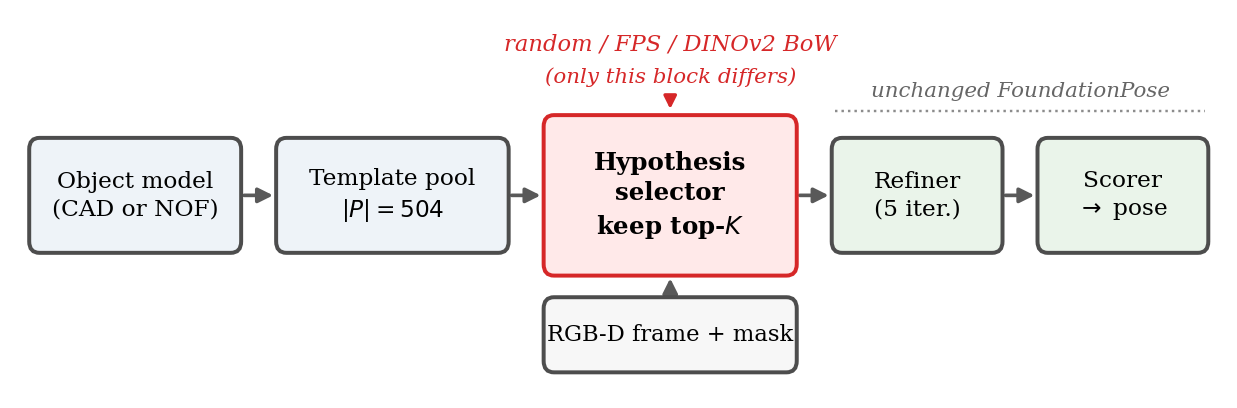
\includegraphics[width=0.92\textwidth]{rfigA_pipeline.png}
\caption{Frame-0 registration pipeline. The object model is rendered once into a pool of 504 templates; a selector keeps $K$ of them as pose hypotheses, which the FoundationPose refiner and scorer process unchanged. Only the selector block differs between the compared methods, which isolates its effect on accuracy and latency.}
\label{fig:pipeline}
\end{figure*}

The proposed selector is geodesic farthest-point sampling (FPS) of the pose pool. The overall pipeline and the position of the selector are shown in Fig.~\ref{fig:pipeline}. Starting from a random template, it uses a greedy strategy that iteratively adds the pose farthest (in rotation) from the already selected set which maximizes angular coverage for a given budget $K$ (Algorithm 1). The rationale is that the refiner corrects a hypothesis only within a limited basin of attraction, so what matters is that some retained hypothesis lies near the true rotation; maximizing coverage of $SO(3)$ maximizes that probability. Unlike appearance-based ranking, FPS uses no image features. FPS itself is a classical sampling algorithm; the contribution here is its formulation as a rotation-space hypothesis selector for a learned render-and-compare refiner, together with the controlled comparison against random and foundation feature selection and the resulting speed--accuracy characterization, none of which has been reported for this pipeline.

\section{Implementation and Measurement}

\subsection{Methodology}
The 504 templates come from 42 icosphere viewpoints combined with 12 distinct in-plane rotations, rendered once per object with differentiable rasterization [11]. For each object and strategy we sweep $K \in \{1, 3, 5, 10, 20, 50\}$ over all 16 frames and log ADD, ADD-S, and end-to-end register time (with GPU synchronization after a warm-up). The full-grid anchor ($K{=}252$) is measured on five representative objects. DINOv2 features are computed and stored once per frame, ensuring that the retrieval branch does not repeat the same calculation. All experiments run on a single NVIDIA Tesla T4 (16 GB) in Google Colab with PyTorch and CUDA 12.1; every configuration uses the same GPU, so the reported speedups are internally consistent. Parameters are listed in Table~\ref{tab:params}; the pool density (42$\times$12) trades coverage against build cost, and five refiner iterations follow the FoundationPose default so that only the hypothesis source varies. Absolute latencies would decrease on a more powerful GPU, where the 252-hypothesis batch is less resource-constrained, so the speedup reported here is specific to this class of hardware.

\begin{table}[tb]
\caption{Parameter Settings}
\label{tab:params}
\centering\small
\begin{tabular}{@{}ll@{}}
\toprule
Parameter & Value \\
\midrule
Template pool ($N_s \times N_i$) & $42 \times 12 = 504$ \\
DINOv2 backbone / layer & ViT-B/14 / layer 9 \\
BoW vocabulary & 256 words, TF-IDF \\
Refiner iterations & 5 \\
$K$ sweep & 1, 3, 5, 10, 20, 50 \\
Objects / frames & 21 / 16 \\
Metric & ADD, ADD-S vs GT ($< 0.1\,d$) \\
\bottomrule
\end{tabular}
\end{table}

\subsection{Results and Discussion}
Fig.~\ref{fig:acc} reports ADD-S recall versus $K$ for the three strategies on the eight objects evaluated with all three selectors, with the full-grid anchor as reference (Table~\ref{tab:decisive} lists the values). FPS approaches the anchor by $K{=}20$; random is close behind; DINOv2 bag-of-words retrieval is consistently below random for $K \ge 5$ (e.g. 78.9\% vs 93.0\% at $K{=}10$). Because bag-of-words discards the spatial arrangement of patches, its similarity metric relies purely on the frequency of visual features rather than viewpoint; for textured boxes and cans many rotations share similar histograms, so the top-$K$ cluster by appearance and cover $SO(3)$ worse than uniform sampling. Farthest point sampling performs better for the opposite reason: it optimizes rotational coverage directly.

\begin{figure}[tb]
\centering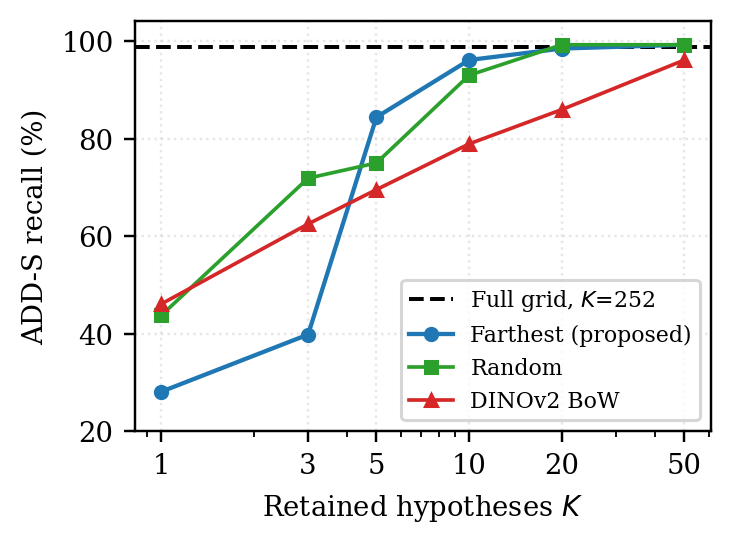
\includegraphics[width=\columnwidth]{rfig1_accuracy.png}
\caption{ADD-S recall versus retained hypotheses $K$ (eight objects, three strategies). Farthest-point sampling approaches the full grid by $K{=}20$; DINOv2 bag-of-words retrieval falls below random for $K \ge 5$.}
\label{fig:acc}
\end{figure}

\begin{table}[tb]
\caption{ADD-S Recall (\%) by Strategy and $K$ (8 objects)}
\label{tab:decisive}
\centering\small
\begin{tabular}{@{}lcccccc@{}}
\toprule
$K$ & 1 & 3 & 5 & 10 & 20 & 50 \\
\midrule
random & 43.8 & 71.9 & 75.0 & 93.0 & 99.2 & 99.2 \\
farthest & 28.1 & 39.8 & 84.4 & 96.1 & 98.4 & 99.2 \\
DINOv2 BoW & 46.1 & 62.5 & 69.5 & 78.9 & 85.9 & 96.1 \\
\bottomrule
\end{tabular}
\end{table}

Table~\ref{tab:decisive} also exposes the crossover between random and farthest sampling. At very small budgets ($K \le 3$) random is better (e.g. 71.9\% vs 39.8\% at $K{=}3$): farthest sampling pushes the first few poses maximally apart and leaves large gaps in the interior of $SO(3)$, whereas random draws are unbiased. From $K \ge 5$ the coverage advantage of farthest sampling dominates and it overtakes random. The same pattern holds on the full 21-object set (Table~\ref{tab:breadth}). These findings establish a practical guideline: use farthest sampling for $K \ge 5$ (practically $K \ge 10$), and random below that.

\begin{table}[tb]
\caption{ADD-S Recall (\%), Random vs Farthest (21 objects)}
\label{tab:breadth}
\centering\small
\begin{tabular}{@{}lcccccc@{}}
\toprule
$K$ & 1 & 3 & 5 & 10 & 20 & 50 \\
\midrule
random & 42.9 & 72.9 & 78.9 & 92.0 & 98.2 & 99.7 \\
farthest & 37.8 & 44.0 & 84.8 & 96.1 & 99.4 & 99.7 \\
\bottomrule
\end{tabular}
\end{table}

Fig.~\ref{fig:time} reports register time. The three strategies cost almost the same because the refiner and scorer account for most of the computational cost. Given that the DINOv2 overhead is minimal, accuracy becomes the primary distinguishing factor rather than speed. DINOv2 retrieval is therefore dominated: at equal $K$ it costs the same time as the geometric selectors but is less accurate, so no latency budget exists at which it is the preferred choice. Time grows linearly, $t \approx 192 + 17.0K$ ms, matching (1).

\begin{figure}[tb]
\centering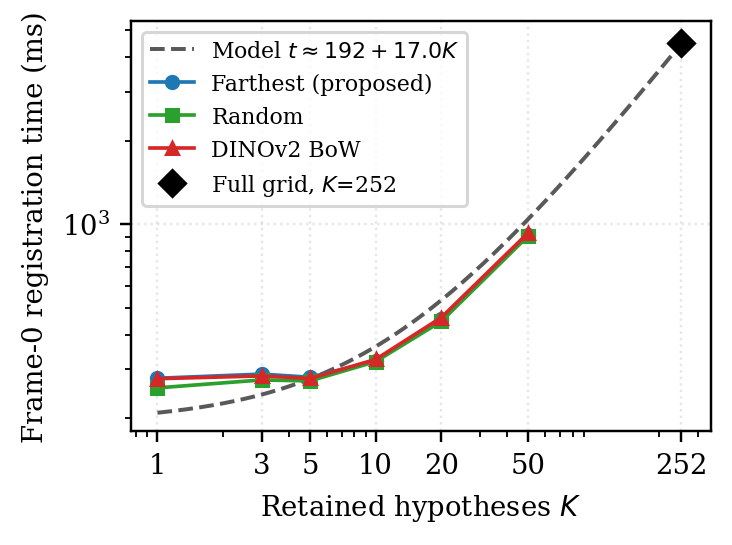
\includegraphics[width=\columnwidth]{rfig2_time.png}
\caption{Frame-0 register time versus $K$ (log--log). All strategies scale as $t \approx 192 + 17.0K$ ms; the full grid ($K{=}252$) costs $\approx 4486$ ms.}
\label{fig:time}
\end{figure}

Fig.~\ref{fig:pareto} shows the speed \& accuracy trade-off over all 21 objects (Table~\ref{tab:summary}). Because the full-grid anchor was measured on five objects, the comparison against it must be made on that same subset; Table~\ref{tab:matched} reports this matched comparison. Farthest-point sampling at $K{=}20$ attains 97.5\% ADD-S at 479 ms against the grid's 98.8\% at 4486 ms, i.e. 9.4 times faster for 1.3 points of ADD-S, and at $K{=}50$ it equals the grid (98.8\%) while still being 4.5$\times$ faster. The five anchor objects deliberately include the two hardest cases, so these figures are a conservative bound; over all 21 objects the same setting reaches 99.4\%.

\begin{figure}[tb]
\centering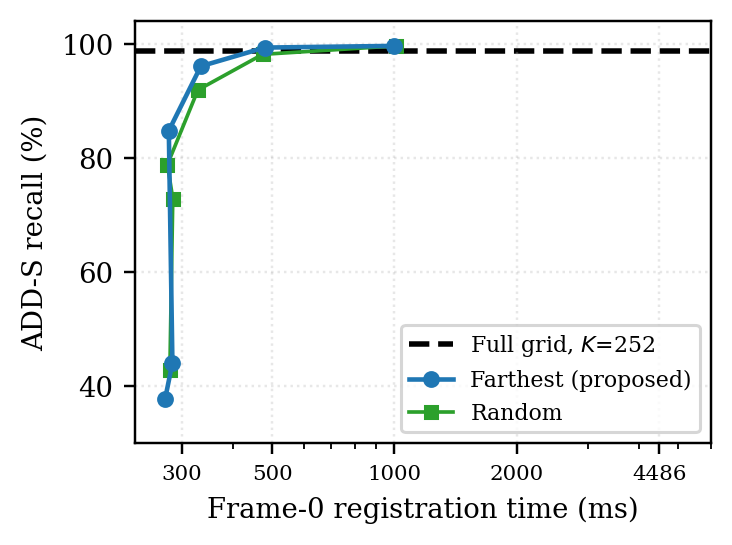
\includegraphics[width=\columnwidth]{rfig3_pareto.png}
\caption{Speed \& accuracy balance over 21 objects. The dashed line marks the full-grid accuracy (98.8\%), reached at 4486 ms; farthest-point sampling reaches its accuracy near $K{=}20$ at a fraction of the time.}
\label{fig:pareto}
\end{figure}

\begin{table}[tb]
\caption{Farthest-Point Sampling, All 21 Objects}
\label{tab:summary}
\centering\small
\begin{tabular}{@{}lccc@{}}
\toprule
Configuration & ADD-S (\%) & Time (ms) & Speedup \\
\midrule
farthest, $K{=}10$ & 96.1 & 334 & $13.4\times$ \\
farthest, $K{=}20$ & 99.4 & 480 & $9.4\times$ \\
farthest, $K{=}50$ & 99.7 & 998 & $4.5\times$ \\
\bottomrule
\end{tabular}
\end{table}

\begin{table}[tb]
\caption{Matched Comparison Against the Full Grid (same 5 objects)}
\label{tab:matched}
\centering\small
\begin{tabular}{@{}lccc@{}}
\toprule
Configuration & ADD-S (\%) & Time (ms) & Speedup \\
\midrule
Full grid, $K{=}252$ & 98.8 & 4486 & $1.0\times$ \\
farthest, $K{=}10$ & 92.5 & 330 & $13.6\times$ \\
farthest, $K{=}20$ & 97.5 & 479 & $9.4\times$ \\
farthest, $K{=}50$ & 98.8 & 1004 & $4.5\times$ \\
\bottomrule
\end{tabular}
\end{table}

Fig.~\ref{fig:perobj} breaks ADD-S down per object at farthest $K{=}20$. Nineteen of 21 objects reach 100\%; the two exceptions are a ``power drill'' (ob15, asymmetric, complex shape) and a ``marker pen'' (ob18, small and nearly cylindrically symmetric), both at 93.8\%. The marker stays near 94\% even at $K{=}50$, so its errors are not a hypothesis-count problem but stem from its small size and few depth points. Over the same 21 objects at $K{=}20$, ADD-S is 99.4\% while ADD is only 69.9\%. This gap reflects symmetry-induced flips, which ADD-S tolerates and ADD does not, and is expected on YCB-Video, where boxes and cans predominate.

\begin{figure}[tb]
\centering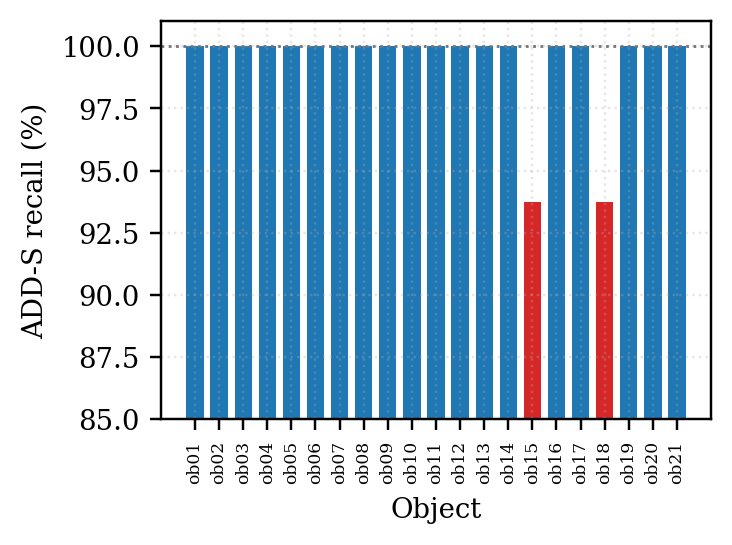
\includegraphics[width=\columnwidth]{rfig4_perobj.png}
\caption{Per-object ADD-S at farthest $K{=}20$. Only the drill (ob15) and marker (ob18) fall below 100\%.}
\label{fig:perobj}
\end{figure}

Table~\ref{tab:perobj} lists the per-object ADD-S at farthest $K{=}10$, $K{=}20$ and $K{=}50$, and at random $K{=}20$. At $K{=}20$ farthest sampling reaches 100\% on 19 of 21 objects; the smallest objects (ob06, ob21 at 9--10 cm) are handled well, so size alone is not the limiting factor. Therefore, small size alone is not the primary limiting factor. Instead, the remaining failure cases occur only when a small physical scale is compounded by rotational symmetry.

\begin{table*}[tb]
\caption{Per-Object ADD-S Recall (\%), 21 Objects. ``far'' = farthest, ``rnd'' = random}
\label{tab:perobj}
\centering\small
\begin{tabular}{@{}lccccc@{\hspace{1.6em}}lccccc@{}}
\toprule
Obj & Diam. & far10 & far20 & far50 & rnd20 & Obj & Diam. & far10 & far20 & far50 & rnd20 \\
\midrule
ob01 & 17.2 & 100.0 & 100.0 & 100.0 & 100.0 & ob12 & 26.0 & 100.0 & 100.0 & 100.0 & 100.0 \\
ob02 & 27.0 & 87.5 & 100.0 & 100.0 & 93.8 & ob13 & 16.2 & 81.2 & 100.0 & 100.0 & 93.8 \\
ob03 & 19.8 & 93.8 & 100.0 & 100.0 & 100.0 & ob14 & 12.5 & 100.0 & 100.0 & 100.0 & 100.0 \\
ob04 & 12.1 & 100.0 & 100.0 & 100.0 & 100.0 & ob15 & 22.6 & 87.5 & 93.8 & 100.0 & 100.0 \\
ob05 & 19.6 & 100.0 & 100.0 & 100.0 & 100.0 & ob16 & 23.7 & 100.0 & 100.0 & 100.0 & 100.0 \\
ob06 & 9.0 & 100.0 & 100.0 & 100.0 & 100.0 & ob17 & 20.4 & 93.8 & 100.0 & 100.0 & 100.0 \\
ob07 & 14.3 & 100.0 & 100.0 & 100.0 & 87.5 & ob18 & 12.1 & 93.8 & \textbf{93.8} & \textbf{93.8} & 93.8 \\
ob08 & 11.4 & 93.8 & 100.0 & 100.0 & 100.0 & ob19 & 17.5 & 100.0 & 100.0 & 100.0 & 100.0 \\
ob09 & 13.0 & 93.8 & 100.0 & 100.0 & 93.8 & ob20 & 21.7 & 100.0 & 100.0 & 100.0 & 100.0 \\
ob10 & 19.8 & 93.8 & 100.0 & 100.0 & 100.0 & ob21 & 10.3 & 100.0 & 100.0 & 100.0 & 100.0 \\
ob11 & 26.0 & 100.0 & 100.0 & 100.0 & 100.0 & & & & & & \\
\midrule
\multicolumn{12}{c}{\textbf{Mean}\quad Diam.\ 17.7\,cm \quad|\quad far10: 96.1 \quad|\quad far20: 99.4 \quad|\quad far50: 99.7 \quad|\quad rnd20: 98.2}\\
\bottomrule
\end{tabular}
\end{table*}

Table~\ref{tab:add} reports the non-symmetric ADD metric for the same runs. On these eight objects ADD is far lower than ADD-S (farthest: 82.8\% vs 98.4\% at $K{=}20$) and the ordering is preserved: FPS outperforms random sampling, which outperforms DINOv2 BoW for $K \ge 5$. The large ADD/ADD-S gap is the signature of $180^{\circ}$ symmetry flips on boxes and cans that are pose-ambiguous from a single view; ADD-S is therefore the correct primary metric under the BOP protocol [10], and the ADD column mainly quantifies how often the refiner resolves the symmetric ambiguity, not selection quality.

\begin{table}[tb]
\caption{ADD Recall (\%, non-symmetric) by Strategy and $K$ (8 objects)}
\label{tab:add}
\centering\small
\begin{tabular}{@{}lcccccc@{}}
\toprule
$K$ & 1 & 3 & 5 & 10 & 20 & 50 \\
\midrule
random & 8.6 & 24.2 & 32.0 & 44.5 & 68.8 & 85.2 \\
farthest & 5.5 & 17.2 & 40.6 & 64.1 & 82.8 & 87.5 \\
DINOv2 BoW & 10.9 & 22.7 & 27.3 & 41.4 & 48.4 & 72.7 \\
\bottomrule
\end{tabular}
\end{table}

For this pipeline the default operating point is farthest-point sampling at $K{=}20$: it comes within 1.3 points of full-grid ADD-S at about nine times lower latency and needs no image features, no learned index, and no per-object offline retrieval build. To maintain accuracy, $K{=}50$ matches the full grid at 4.5 times faster; when latency is critical, $K{=}10$ gives a further speedup to 13 times at a larger accuracy cost.

\subsection{Discussion}
The DINOv2 selector evaluated here ranks templates by a bag-of-words vector, which discards the spatial layout of patches. FoundPose [4] and GigaPose [7] additionally establish 2D--3D patch correspondences and solve Perspective-$n$-Point, retaining geometry; our negative result applies to the bag-of-words variant specifically. It does not necessarily extend to correspondence-based selectors such as FoundPose [4] or GigaPose [7]. However, any such selector must still propose rotation hypotheses, and unless it improves coverage of the true rotation over a geometric baseline, it cannot outperform farthest sampling once the refiner resolves nearby initializations.

The refiner has a finite convergence region: it converges when a hypothesis lies within a limited angular distance of the truth and fails otherwise. Accuracy is then governed by the probability that at least one retained hypothesis falls inside that region, i.e., by the covering radius of the retained set on $SO(3)$. FPS directly optimizes the rotational coverage. In contrast, the retrieval method focuses on a separate objective centered on feature similarity, which is only weakly correlated with rotation and is nearly uninformative for textured or symmetric objects. This accounts for both the advantage of farthest sampling and the below-random behavior of bag-of-words retrieval. Fig.~\ref{fig:coverage} measures this directly on the 504-pose pool.

\begin{figure}[tb]
\centering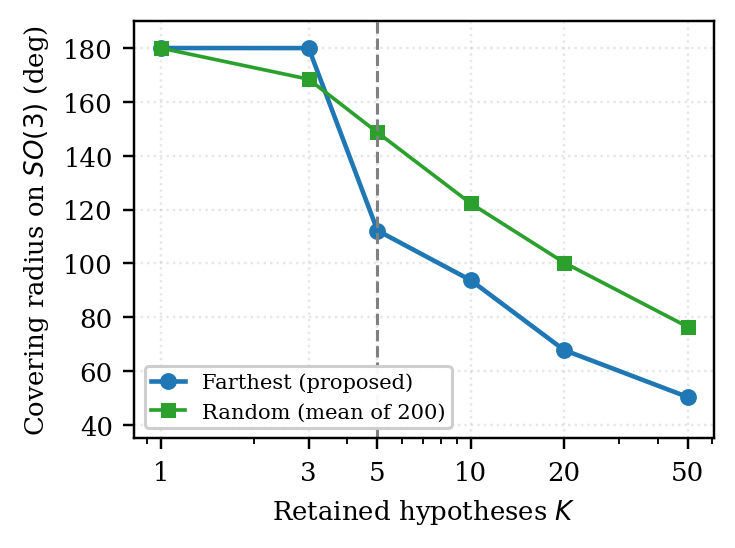
\includegraphics[width=\columnwidth]{rfigB_coverage.png}
\caption{Covering radius of the retained hypothesis set on $SO(3)$: the largest geodesic angle from an arbitrary rotation to its nearest retained hypothesis (lower is better). Farthest sampling overtakes random selection at $K{=}5$ (dashed line), matching the accuracy crossover.}
\label{fig:coverage}
\end{figure}

The pool, refiner, and metric are those of FoundationPose, so the experimental numbers are specific to render-and-compare with a strongly learned refiner. The linear time model and the covering-radius argument are generalizable to other pipelines and should transfer to any method that refines and scores a discrete hypothesis set.

Absolute timings are specific to the Tesla T4 used here and are reported as ratios where possible; on a stronger GPU the 252-hypothesis batch parallelizes better and the speedup would shrink. The full-grid anchor is measured on five objects, so all comparisons against it are made on that matched subset (Table~\ref{tab:matched}) rather than against the 21-object mean; because those five include the two hardest objects, the matched figures understate average performance. All data come from YCB-Video, where boxes and cans predominate, so the symmetry statistics may not transfer to thin or articulated objects. The true pose convention is auto-detected and verified against the full-grid output before evaluation, and runs with poor agreement are rejected.

\section{Conclusion}
For FoundationPose first-frame registration, most of the 252-hypothesis grid is redundant. Selecting hypotheses by geodesic farthest-point sampling reaches 97.5\% ADD-S against the full grid's 98.8\% at $K{=}20$ on a matched object set, about nine times faster, and equals the grid at $K{=}50$ while still being 4.5 times faster; register time follows $t \approx 192 + 17.0K$ ms. A DINOv2 bag-of-words retrieval selector underperforms even random selection, because bag-of-words ranking is viewpoint-independent; for hypotheses feeding a strong render-and-compare refiner, coverage of the rotation space matters more than appearance ranking. The recommended configuration is farthest-point sampling with $K \in [10, 20]$; random selection is preferable below $K{=}5$. Limitations include evaluation on YCB-Video only, timings measured on a single Tesla T4, a full-grid anchor computed on five objects, and residual errors on small or symmetric objects. Future work includes correspondence-based (PnP) selection as an alternative to bag-of-words, model-free objects, and mask-free initialization.

\section*{References}
\begin{enumerate}\small\itemsep1pt\parskip0pt
\item B. Wen, W. Yang, J. Kautz, and S. Birchfield, ``FoundationPose: Unified 6D pose estimation and tracking of novel objects,'' in Proc. IEEE/CVF CVPR, 2024.
\item Y. Labbé, L. Manuelli, A. Mousavian, et al., ``MegaPose: 6D pose estimation of novel objects via render and compare,'' in Proc. CoRL, 2022.
\item B. Wen, J. Tremblay, V. Blukis, et al., ``BundleSDF: Neural 6-DoF tracking and 3D reconstruction of unknown objects,'' in Proc. IEEE/CVF CVPR, 2023.
\item E. P. Örnek, Y. Labbé, B. Tekin, et al., ``FoundPose: Unsupervised deep pose estimation using foundation features,'' in Proc. ECCV, 2024.
\item M. Oquab, T. Darcet, T. Moutakanni, et al., ``DINOv2: Learning robust visual features without supervision,'' Trans. Mach. Learn. Res., 2024.
\item J. Sivic and A. Zisserman, ``Video Google: A text retrieval approach to object matching in videos,'' in Proc. IEEE ICCV, 2003.
\item V. N. Nguyen, T. Groueix, M. Salzmann, and V. Lepetit, ``GigaPose: Fast and robust novel object pose estimation via one correspondence,'' in Proc. IEEE/CVF CVPR, 2024.
\item S. Hinterstoisser, V. Lepetit, S. Ilic, et al., ``Model based training, detection and pose estimation of texture-less 3D objects in heavily cluttered scenes,'' in Proc. ACCV, 2012.
\item Y. Xiang, T. Schmidt, V. Narayanan, and D. Fox, ``PoseCNN: A convolutional neural network for 6D object pose estimation in cluttered scenes,'' in Proc. RSS, 2018.
\item T. Hodaň, F. Michel, E. Brachmann, et al., ``BOP: Benchmark for 6D object pose estimation,'' in Proc. ECCV, 2018.
\item S. Laine, J. Hellsten, T. Karras, et al., ``Modular primitives for high-performance differentiable rendering,'' ACM Trans. Graph., vol. 39, no. 6, 2020.
\end{enumerate}

\end{document}
